% !TEX encoding = UTF-8 Unicode
\documentclass[10pt]{standalone}\usepackage{tikz,graphicx}
\usepackage{fontspec}
\setmainfont{Arial}
\setsansfont{Arial}\begin{document}

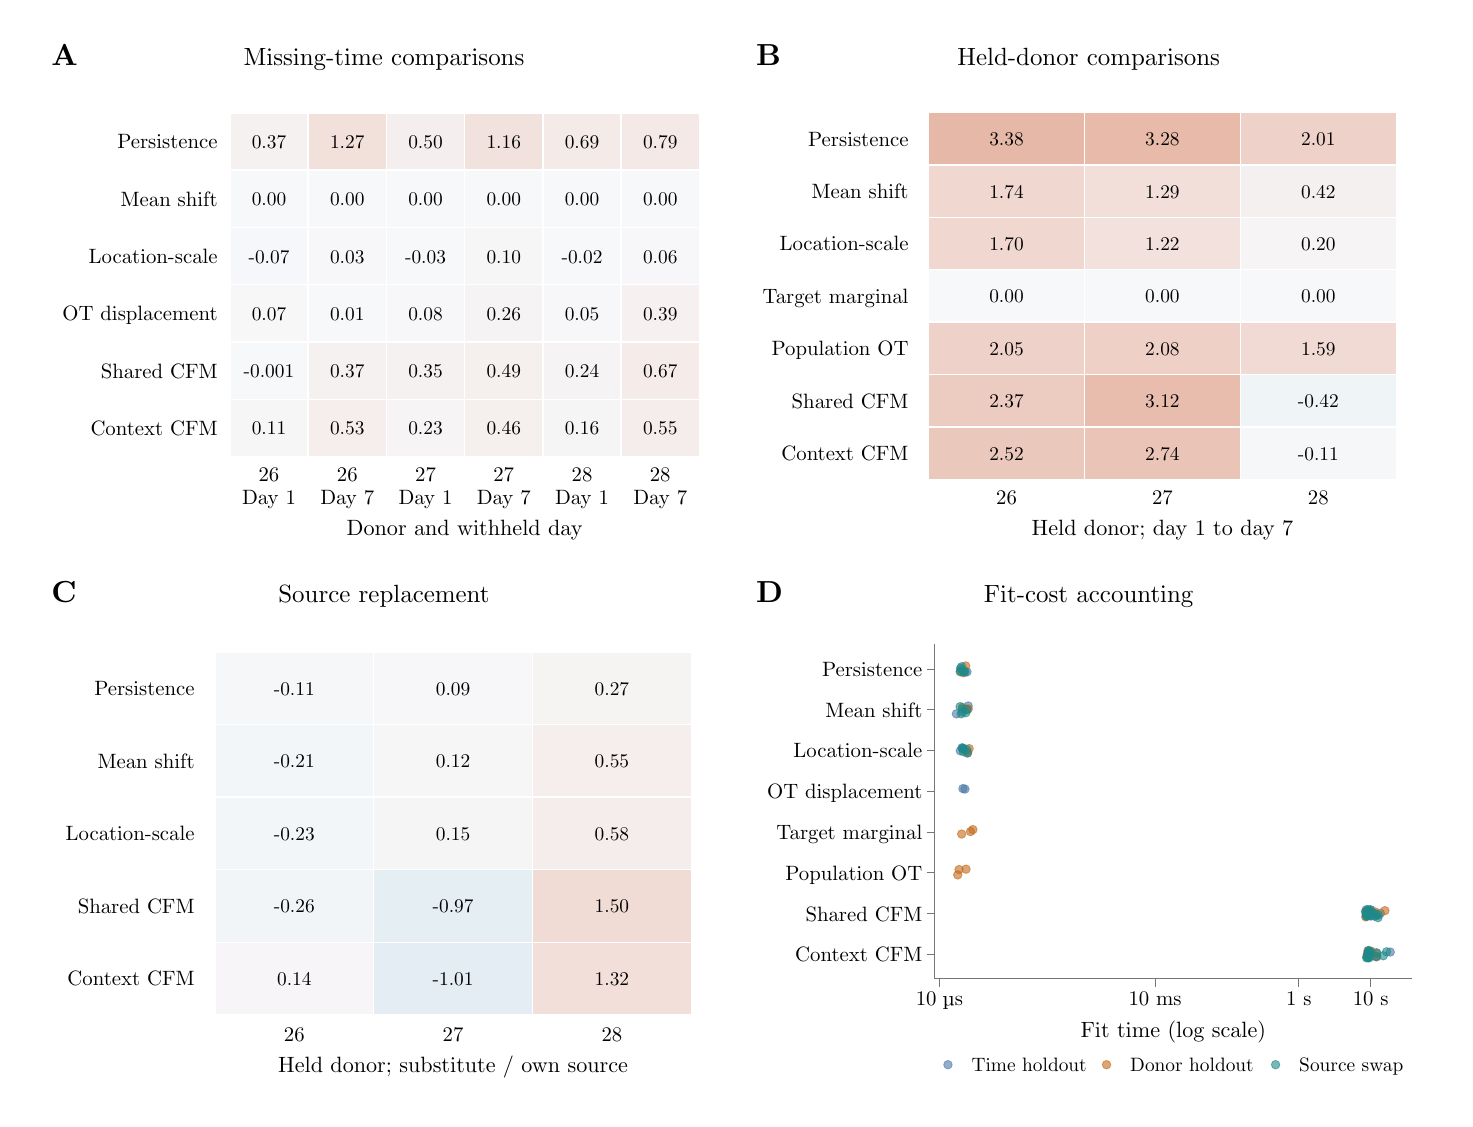
\begin{tikzpicture}[x=1pt,y=1pt]
\definecolor{fillColor}{RGB}{255,255,255}
\path[use as bounding box,fill=fillColor,fill opacity=0.00] (0,0) rectangle (512.15,386.96);
\begin{scope}
\path[clip] (  0.00,  0.00) rectangle (512.15,386.96);
\definecolor{drawColor}{RGB}{0,0,0}

\node[text=drawColor,anchor=base west,inner sep=0pt, outer sep=0pt, scale=  1.10] at (  8.54,373.39) {\bfseries A};

\node[text=drawColor,anchor=base,inner sep=0pt, outer sep=0pt, scale=  0.90] at (128.75,373.40) {Missing-time comparisons};
\end{scope}
\begin{scope}
\path[clip] (  8.54,198.46) rectangle (248.96,363.34);
\definecolor{fillColor}{RGB}{255,255,255}

\path[fill=fillColor] (  8.54,198.46) rectangle (248.96,363.34);
\end{scope}
\begin{scope}
\path[clip] ( 70.24,229.91) rectangle (245.55,358.22);
\definecolor{fillColor}{RGB}{255,255,255}

\path[fill=fillColor] ( 70.24,229.91) rectangle (245.55,358.22);
\definecolor{drawColor}{RGB}{255,255,255}
\definecolor{fillColor}{RGB}{247,246,247}

\path[draw=drawColor,line width= 0.5pt,fill=fillColor] ( 73.07,231.98) rectangle (101.34,252.68);
\definecolor{fillColor}{RGB}{246,244,244}

\path[draw=drawColor,line width= 0.5pt,fill=fillColor] (129.62,231.98) rectangle (157.89,252.68);
\definecolor{fillColor}{RGB}{246,245,246}

\path[draw=drawColor,line width= 0.5pt,fill=fillColor] (186.17,231.98) rectangle (214.44,252.68);
\definecolor{fillColor}{RGB}{247,248,250}

\path[draw=drawColor,line width= 0.5pt,fill=fillColor] ( 73.07,252.68) rectangle (101.34,273.37);
\definecolor{fillColor}{RGB}{246,241,241}

\path[draw=drawColor,line width= 0.5pt,fill=fillColor] (129.62,252.68) rectangle (157.89,273.37);
\definecolor{fillColor}{RGB}{246,243,244}

\path[draw=drawColor,line width= 0.5pt,fill=fillColor] (186.17,252.68) rectangle (214.44,273.37);
\definecolor{fillColor}{RGB}{246,241,241}

\path[draw=drawColor,line width= 0.5pt,fill=fillColor] ( 73.07,335.46) rectangle (101.34,356.15);
\definecolor{fillColor}{RGB}{245,238,238}

\path[draw=drawColor,line width= 0.5pt,fill=fillColor] (129.62,335.46) rectangle (157.89,356.15);
\definecolor{fillColor}{RGB}{244,235,233}

\path[draw=drawColor,line width= 0.5pt,fill=fillColor] (186.17,335.46) rectangle (214.44,356.15);
\definecolor{fillColor}{RGB}{246,247,250}

\path[draw=drawColor,line width= 0.5pt,fill=fillColor] ( 73.07,294.07) rectangle (101.34,314.76);
\definecolor{fillColor}{RGB}{246,248,250}

\path[draw=drawColor,line width= 0.5pt,fill=fillColor] (129.62,294.07) rectangle (157.89,314.76);
\definecolor{fillColor}{RGB}{247,248,250}

\path[draw=drawColor,line width= 0.5pt,fill=fillColor] (186.17,294.07) rectangle (214.44,314.76);

\path[draw=drawColor,line width= 0.5pt,fill=fillColor] ( 73.07,314.76) rectangle (101.34,335.46);

\path[draw=drawColor,line width= 0.5pt,fill=fillColor] (129.62,314.76) rectangle (157.89,335.46);

\path[draw=drawColor,line width= 0.5pt,fill=fillColor] (186.17,314.76) rectangle (214.44,335.46);
\definecolor{fillColor}{RGB}{247,247,248}

\path[draw=drawColor,line width= 0.5pt,fill=fillColor] ( 73.07,273.37) rectangle (101.34,294.07);
\definecolor{fillColor}{RGB}{247,246,248}

\path[draw=drawColor,line width= 0.5pt,fill=fillColor] (129.62,273.37) rectangle (157.89,294.07);
\definecolor{fillColor}{RGB}{247,247,249}

\path[draw=drawColor,line width= 0.5pt,fill=fillColor] (186.17,273.37) rectangle (214.44,294.07);
\definecolor{fillColor}{RGB}{245,238,237}

\path[draw=drawColor,line width= 0.5pt,fill=fillColor] (101.34,231.98) rectangle (129.62,252.68);
\definecolor{fillColor}{RGB}{245,239,238}

\path[draw=drawColor,line width= 0.5pt,fill=fillColor] (157.89,231.98) rectangle (186.17,252.68);
\definecolor{fillColor}{RGB}{245,237,236}

\path[draw=drawColor,line width= 0.5pt,fill=fillColor] (214.44,231.98) rectangle (242.72,252.68);
\definecolor{fillColor}{RGB}{246,241,241}

\path[draw=drawColor,line width= 0.5pt,fill=fillColor] (101.34,252.68) rectangle (129.62,273.37);
\definecolor{fillColor}{RGB}{245,239,238}

\path[draw=drawColor,line width= 0.5pt,fill=fillColor] (157.89,252.68) rectangle (186.17,273.37);
\definecolor{fillColor}{RGB}{245,235,233}

\path[draw=drawColor,line width= 0.5pt,fill=fillColor] (214.44,252.68) rectangle (242.72,273.37);
\definecolor{fillColor}{RGB}{242,224,219}

\path[draw=drawColor,line width= 0.5pt,fill=fillColor] (101.34,335.46) rectangle (129.62,356.15);
\definecolor{fillColor}{RGB}{242,226,221}

\path[draw=drawColor,line width= 0.5pt,fill=fillColor] (157.89,335.46) rectangle (186.17,356.15);
\definecolor{fillColor}{RGB}{244,233,230}

\path[draw=drawColor,line width= 0.5pt,fill=fillColor] (214.44,335.46) rectangle (242.72,356.15);
\definecolor{fillColor}{RGB}{247,247,249}

\path[draw=drawColor,line width= 0.5pt,fill=fillColor] (101.34,294.07) rectangle (129.62,314.76);
\definecolor{fillColor}{RGB}{247,246,247}

\path[draw=drawColor,line width= 0.5pt,fill=fillColor] (157.89,294.07) rectangle (186.17,314.76);
\definecolor{fillColor}{RGB}{247,247,249}

\path[draw=drawColor,line width= 0.5pt,fill=fillColor] (214.44,294.07) rectangle (242.72,314.76);
\definecolor{fillColor}{RGB}{247,248,250}

\path[draw=drawColor,line width= 0.5pt,fill=fillColor] (101.34,314.76) rectangle (129.62,335.46);

\path[draw=drawColor,line width= 0.5pt,fill=fillColor] (157.89,314.76) rectangle (186.17,335.46);

\path[draw=drawColor,line width= 0.5pt,fill=fillColor] (214.44,314.76) rectangle (242.72,335.46);

\path[draw=drawColor,line width= 0.5pt,fill=fillColor] (101.34,273.37) rectangle (129.62,294.07);
\definecolor{fillColor}{RGB}{246,243,244}

\path[draw=drawColor,line width= 0.5pt,fill=fillColor] (157.89,273.37) rectangle (186.17,294.07);
\definecolor{fillColor}{RGB}{246,241,240}

\path[draw=drawColor,line width= 0.5pt,fill=fillColor] (214.44,273.37) rectangle (242.72,294.07);
\definecolor{drawColor}{RGB}{0,0,0}

\node[text=drawColor,anchor=base,inner sep=0pt, outer sep=0pt, scale=  0.70] at ( 87.20,239.82) {0.11};

\node[text=drawColor,anchor=base,inner sep=0pt, outer sep=0pt, scale=  0.70] at (143.76,239.82) {0.23};

\node[text=drawColor,anchor=base,inner sep=0pt, outer sep=0pt, scale=  0.70] at (200.31,239.82) {0.16};

\node[text=drawColor,anchor=base,inner sep=0pt, outer sep=0pt, scale=  0.70] at ( 87.20,260.52) {-0.001};

\node[text=drawColor,anchor=base,inner sep=0pt, outer sep=0pt, scale=  0.70] at (143.76,260.52) {0.35};

\node[text=drawColor,anchor=base,inner sep=0pt, outer sep=0pt, scale=  0.70] at (200.31,260.52) {0.24};

\node[text=drawColor,anchor=base,inner sep=0pt, outer sep=0pt, scale=  0.70] at ( 87.20,343.30) {0.37};

\node[text=drawColor,anchor=base,inner sep=0pt, outer sep=0pt, scale=  0.70] at (143.76,343.30) {0.50};

\node[text=drawColor,anchor=base,inner sep=0pt, outer sep=0pt, scale=  0.70] at (200.31,343.30) {0.69};

\node[text=drawColor,anchor=base,inner sep=0pt, outer sep=0pt, scale=  0.70] at ( 87.20,301.91) {-0.07};

\node[text=drawColor,anchor=base,inner sep=0pt, outer sep=0pt, scale=  0.70] at (143.76,301.91) {-0.03};

\node[text=drawColor,anchor=base,inner sep=0pt, outer sep=0pt, scale=  0.70] at (200.31,301.91) {-0.02};

\node[text=drawColor,anchor=base,inner sep=0pt, outer sep=0pt, scale=  0.70] at ( 87.20,322.60) {0.00};

\node[text=drawColor,anchor=base,inner sep=0pt, outer sep=0pt, scale=  0.70] at (143.76,322.60) {0.00};

\node[text=drawColor,anchor=base,inner sep=0pt, outer sep=0pt, scale=  0.70] at (200.31,322.60) {0.00};

\node[text=drawColor,anchor=base,inner sep=0pt, outer sep=0pt, scale=  0.70] at ( 87.20,281.21) {0.07};

\node[text=drawColor,anchor=base,inner sep=0pt, outer sep=0pt, scale=  0.70] at (143.76,281.21) {0.08};

\node[text=drawColor,anchor=base,inner sep=0pt, outer sep=0pt, scale=  0.70] at (200.31,281.21) {0.05};

\node[text=drawColor,anchor=base,inner sep=0pt, outer sep=0pt, scale=  0.70] at (115.48,239.82) {0.53};

\node[text=drawColor,anchor=base,inner sep=0pt, outer sep=0pt, scale=  0.70] at (172.03,239.82) {0.46};

\node[text=drawColor,anchor=base,inner sep=0pt, outer sep=0pt, scale=  0.70] at (228.58,239.82) {0.55};

\node[text=drawColor,anchor=base,inner sep=0pt, outer sep=0pt, scale=  0.70] at (115.48,260.52) {0.37};

\node[text=drawColor,anchor=base,inner sep=0pt, outer sep=0pt, scale=  0.70] at (172.03,260.52) {0.49};

\node[text=drawColor,anchor=base,inner sep=0pt, outer sep=0pt, scale=  0.70] at (228.58,260.52) {0.67};

\node[text=drawColor,anchor=base,inner sep=0pt, outer sep=0pt, scale=  0.70] at (115.48,343.30) {1.27};

\node[text=drawColor,anchor=base,inner sep=0pt, outer sep=0pt, scale=  0.70] at (172.03,343.30) {1.16};

\node[text=drawColor,anchor=base,inner sep=0pt, outer sep=0pt, scale=  0.70] at (228.58,343.30) {0.79};

\node[text=drawColor,anchor=base,inner sep=0pt, outer sep=0pt, scale=  0.70] at (115.48,301.91) {0.03};

\node[text=drawColor,anchor=base,inner sep=0pt, outer sep=0pt, scale=  0.70] at (172.03,301.91) {0.10};

\node[text=drawColor,anchor=base,inner sep=0pt, outer sep=0pt, scale=  0.70] at (228.58,301.91) {0.06};

\node[text=drawColor,anchor=base,inner sep=0pt, outer sep=0pt, scale=  0.70] at (115.48,322.60) {0.00};

\node[text=drawColor,anchor=base,inner sep=0pt, outer sep=0pt, scale=  0.70] at (172.03,322.60) {0.00};

\node[text=drawColor,anchor=base,inner sep=0pt, outer sep=0pt, scale=  0.70] at (228.58,322.60) {0.00};

\node[text=drawColor,anchor=base,inner sep=0pt, outer sep=0pt, scale=  0.70] at (115.48,281.21) {0.01};

\node[text=drawColor,anchor=base,inner sep=0pt, outer sep=0pt, scale=  0.70] at (172.03,281.21) {0.26};

\node[text=drawColor,anchor=base,inner sep=0pt, outer sep=0pt, scale=  0.70] at (228.58,281.21) {0.39};
\end{scope}
\begin{scope}
\path[clip] (  0.00,  0.00) rectangle (512.15,386.96);
\definecolor{drawColor}{RGB}{0,0,0}

\node[text=drawColor,anchor=base east,inner sep=0pt, outer sep=0pt, scale=  0.75] at ( 68.64,239.65) {Context CFM};

\node[text=drawColor,anchor=base east,inner sep=0pt, outer sep=0pt, scale=  0.75] at ( 68.64,260.34) {Shared CFM};

\node[text=drawColor,anchor=base east,inner sep=0pt, outer sep=0pt, scale=  0.75] at ( 68.64,281.03) {OT displacement};

\node[text=drawColor,anchor=base east,inner sep=0pt, outer sep=0pt, scale=  0.75] at ( 68.64,301.73) {Location-scale};

\node[text=drawColor,anchor=base east,inner sep=0pt, outer sep=0pt, scale=  0.75] at ( 68.64,322.42) {Mean shift};

\node[text=drawColor,anchor=base east,inner sep=0pt, outer sep=0pt, scale=  0.75] at ( 68.64,343.12) {Persistence};
\end{scope}
\begin{scope}
\path[clip] (  0.00,  0.00) rectangle (512.15,386.96);
\definecolor{drawColor}{RGB}{0,0,0}

\node[text=drawColor,anchor=base,inner sep=0pt, outer sep=0pt, scale=  0.75] at ( 87.20,222.94) {26};

\node[text=drawColor,anchor=base,inner sep=0pt, outer sep=0pt, scale=  0.75] at ( 87.20,214.84) {Day 1};

\node[text=drawColor,anchor=base,inner sep=0pt, outer sep=0pt, scale=  0.75] at (115.48,222.94) {26};

\node[text=drawColor,anchor=base,inner sep=0pt, outer sep=0pt, scale=  0.75] at (115.48,214.84) {Day 7};

\node[text=drawColor,anchor=base,inner sep=0pt, outer sep=0pt, scale=  0.75] at (143.76,222.94) {27};

\node[text=drawColor,anchor=base,inner sep=0pt, outer sep=0pt, scale=  0.75] at (143.76,214.84) {Day 1};

\node[text=drawColor,anchor=base,inner sep=0pt, outer sep=0pt, scale=  0.75] at (172.03,222.94) {27};

\node[text=drawColor,anchor=base,inner sep=0pt, outer sep=0pt, scale=  0.75] at (172.03,214.84) {Day 7};

\node[text=drawColor,anchor=base,inner sep=0pt, outer sep=0pt, scale=  0.75] at (200.31,222.94) {28};

\node[text=drawColor,anchor=base,inner sep=0pt, outer sep=0pt, scale=  0.75] at (200.31,214.84) {Day 1};

\node[text=drawColor,anchor=base,inner sep=0pt, outer sep=0pt, scale=  0.75] at (228.58,222.94) {28};

\node[text=drawColor,anchor=base,inner sep=0pt, outer sep=0pt, scale=  0.75] at (228.58,214.84) {Day 7};
\end{scope}
\begin{scope}
\path[clip] (  0.00,  0.00) rectangle (512.15,386.96);
\definecolor{drawColor}{RGB}{0,0,0}

\node[text=drawColor,anchor=base,inner sep=0pt, outer sep=0pt, scale=  0.80] at (157.89,203.56) {Donor and withheld day};
\end{scope}
\begin{scope}
\path[clip] (  0.00,  0.00) rectangle (512.15,386.96);
\definecolor{drawColor}{RGB}{0,0,0}

\node[text=drawColor,anchor=base west,inner sep=0pt, outer sep=0pt, scale=  1.10] at (263.19,373.39) {\bfseries B};

\node[text=drawColor,anchor=base,inner sep=0pt, outer sep=0pt, scale=  0.90] at (383.40,373.40) {Held-donor comparisons};
\end{scope}
\begin{scope}
\path[clip] (263.19,198.46) rectangle (503.61,363.34);
\definecolor{fillColor}{RGB}{255,255,255}

\path[fill=fillColor] (263.19,198.46) rectangle (503.61,363.34);
\end{scope}
\begin{scope}
\path[clip] (319.89,221.81) rectangle (500.20,358.22);
\definecolor{fillColor}{RGB}{255,255,255}

\path[fill=fillColor] (319.89,221.81) rectangle (500.20,358.22);
\definecolor{drawColor}{RGB}{255,255,255}
\definecolor{fillColor}{RGB}{245,247,249}

\path[draw=drawColor,line width= 0.5pt,fill=fillColor] (438.22,223.71) rectangle (494.56,242.65);
\definecolor{fillColor}{RGB}{239,244,247}

\path[draw=drawColor,line width= 0.5pt,fill=fillColor] (438.22,242.65) rectangle (494.56,261.60);
\definecolor{fillColor}{RGB}{238,210,201}

\path[draw=drawColor,line width= 0.5pt,fill=fillColor] (438.22,337.38) rectangle (494.56,356.33);
\definecolor{fillColor}{RGB}{246,244,245}

\path[draw=drawColor,line width= 0.5pt,fill=fillColor] (438.22,299.49) rectangle (494.56,318.43);
\definecolor{fillColor}{RGB}{245,240,240}

\path[draw=drawColor,line width= 0.5pt,fill=fillColor] (438.22,318.43) rectangle (494.56,337.38);
\definecolor{fillColor}{RGB}{240,218,211}

\path[draw=drawColor,line width= 0.5pt,fill=fillColor] (438.22,261.60) rectangle (494.56,280.54);
\definecolor{fillColor}{RGB}{247,248,250}

\path[draw=drawColor,line width= 0.5pt,fill=fillColor] (438.22,280.54) rectangle (494.56,299.49);
\definecolor{fillColor}{RGB}{235,200,188}

\path[draw=drawColor,line width= 0.5pt,fill=fillColor] (325.53,223.71) rectangle (381.87,242.65);
\definecolor{fillColor}{RGB}{236,203,192}

\path[draw=drawColor,line width= 0.5pt,fill=fillColor] (325.53,242.65) rectangle (381.87,261.60);
\definecolor{fillColor}{RGB}{230,184,168}

\path[draw=drawColor,line width= 0.5pt,fill=fillColor] (325.53,337.38) rectangle (381.87,356.33);
\definecolor{fillColor}{RGB}{240,216,208}

\path[draw=drawColor,line width= 0.5pt,fill=fillColor] (325.53,299.49) rectangle (381.87,318.43);
\definecolor{fillColor}{RGB}{240,215,207}

\path[draw=drawColor,line width= 0.5pt,fill=fillColor] (325.53,318.43) rectangle (381.87,337.38);
\definecolor{fillColor}{RGB}{238,209,200}

\path[draw=drawColor,line width= 0.5pt,fill=fillColor] (325.53,261.60) rectangle (381.87,280.54);
\definecolor{fillColor}{RGB}{247,248,250}

\path[draw=drawColor,line width= 0.5pt,fill=fillColor] (325.53,280.54) rectangle (381.87,299.49);
\definecolor{fillColor}{RGB}{234,196,183}

\path[draw=drawColor,line width= 0.5pt,fill=fillColor] (381.87,223.71) rectangle (438.22,242.65);
\definecolor{fillColor}{RGB}{232,189,174}

\path[draw=drawColor,line width= 0.5pt,fill=fillColor] (381.87,242.65) rectangle (438.22,261.60);
\definecolor{fillColor}{RGB}{231,186,170}

\path[draw=drawColor,line width= 0.5pt,fill=fillColor] (381.87,337.38) rectangle (438.22,356.33);
\definecolor{fillColor}{RGB}{242,225,220}

\path[draw=drawColor,line width= 0.5pt,fill=fillColor] (381.87,299.49) rectangle (438.22,318.43);
\definecolor{fillColor}{RGB}{242,223,218}

\path[draw=drawColor,line width= 0.5pt,fill=fillColor] (381.87,318.43) rectangle (438.22,337.38);
\definecolor{fillColor}{RGB}{238,208,199}

\path[draw=drawColor,line width= 0.5pt,fill=fillColor] (381.87,261.60) rectangle (438.22,280.54);
\definecolor{fillColor}{RGB}{247,248,250}

\path[draw=drawColor,line width= 0.5pt,fill=fillColor] (381.87,280.54) rectangle (438.22,299.49);
\definecolor{drawColor}{RGB}{0,0,0}

\node[text=drawColor,anchor=base,inner sep=0pt, outer sep=0pt, scale=  0.70] at (466.39,230.67) {-0.11};

\node[text=drawColor,anchor=base,inner sep=0pt, outer sep=0pt, scale=  0.70] at (466.39,249.62) {-0.42};

\node[text=drawColor,anchor=base,inner sep=0pt, outer sep=0pt, scale=  0.70] at (466.39,344.35) {2.01};

\node[text=drawColor,anchor=base,inner sep=0pt, outer sep=0pt, scale=  0.70] at (466.39,306.46) {0.20};

\node[text=drawColor,anchor=base,inner sep=0pt, outer sep=0pt, scale=  0.70] at (466.39,325.40) {0.42};

\node[text=drawColor,anchor=base,inner sep=0pt, outer sep=0pt, scale=  0.70] at (466.39,268.57) {1.59};

\node[text=drawColor,anchor=base,inner sep=0pt, outer sep=0pt, scale=  0.70] at (466.39,287.51) {0.00};

\node[text=drawColor,anchor=base,inner sep=0pt, outer sep=0pt, scale=  0.70] at (353.70,230.67) {2.52};

\node[text=drawColor,anchor=base,inner sep=0pt, outer sep=0pt, scale=  0.70] at (353.70,249.62) {2.37};

\node[text=drawColor,anchor=base,inner sep=0pt, outer sep=0pt, scale=  0.70] at (353.70,344.35) {3.38};

\node[text=drawColor,anchor=base,inner sep=0pt, outer sep=0pt, scale=  0.70] at (353.70,306.46) {1.70};

\node[text=drawColor,anchor=base,inner sep=0pt, outer sep=0pt, scale=  0.70] at (353.70,325.40) {1.74};

\node[text=drawColor,anchor=base,inner sep=0pt, outer sep=0pt, scale=  0.70] at (353.70,268.57) {2.05};

\node[text=drawColor,anchor=base,inner sep=0pt, outer sep=0pt, scale=  0.70] at (353.70,287.51) {0.00};

\node[text=drawColor,anchor=base,inner sep=0pt, outer sep=0pt, scale=  0.70] at (410.05,230.67) {2.74};

\node[text=drawColor,anchor=base,inner sep=0pt, outer sep=0pt, scale=  0.70] at (410.05,249.62) {3.12};

\node[text=drawColor,anchor=base,inner sep=0pt, outer sep=0pt, scale=  0.70] at (410.05,344.35) {3.28};

\node[text=drawColor,anchor=base,inner sep=0pt, outer sep=0pt, scale=  0.70] at (410.05,306.46) {1.22};

\node[text=drawColor,anchor=base,inner sep=0pt, outer sep=0pt, scale=  0.70] at (410.05,325.40) {1.29};

\node[text=drawColor,anchor=base,inner sep=0pt, outer sep=0pt, scale=  0.70] at (410.05,268.57) {2.08};

\node[text=drawColor,anchor=base,inner sep=0pt, outer sep=0pt, scale=  0.70] at (410.05,287.51) {0.00};
\end{scope}
\begin{scope}
\path[clip] (  0.00,  0.00) rectangle (512.15,386.96);
\definecolor{drawColor}{RGB}{0,0,0}

\node[text=drawColor,anchor=base east,inner sep=0pt, outer sep=0pt, scale=  0.75] at (318.29,230.50) {Context CFM};

\node[text=drawColor,anchor=base east,inner sep=0pt, outer sep=0pt, scale=  0.75] at (318.29,249.44) {Shared CFM};

\node[text=drawColor,anchor=base east,inner sep=0pt, outer sep=0pt, scale=  0.75] at (318.29,268.39) {Population OT};

\node[text=drawColor,anchor=base east,inner sep=0pt, outer sep=0pt, scale=  0.75] at (318.29,287.33) {Target marginal};

\node[text=drawColor,anchor=base east,inner sep=0pt, outer sep=0pt, scale=  0.75] at (318.29,306.28) {Location-scale};

\node[text=drawColor,anchor=base east,inner sep=0pt, outer sep=0pt, scale=  0.75] at (318.29,325.22) {Mean shift};

\node[text=drawColor,anchor=base east,inner sep=0pt, outer sep=0pt, scale=  0.75] at (318.29,344.17) {Persistence};
\end{scope}
\begin{scope}
\path[clip] (  0.00,  0.00) rectangle (512.15,386.96);
\definecolor{drawColor}{RGB}{0,0,0}

\node[text=drawColor,anchor=base,inner sep=0pt, outer sep=0pt, scale=  0.75] at (353.70,214.84) {26};

\node[text=drawColor,anchor=base,inner sep=0pt, outer sep=0pt, scale=  0.75] at (410.05,214.84) {27};

\node[text=drawColor,anchor=base,inner sep=0pt, outer sep=0pt, scale=  0.75] at (466.39,214.84) {28};
\end{scope}
\begin{scope}
\path[clip] (  0.00,  0.00) rectangle (512.15,386.96);
\definecolor{drawColor}{RGB}{0,0,0}

\node[text=drawColor,anchor=base,inner sep=0pt, outer sep=0pt, scale=  0.80] at (410.05,203.56) {Held donor; day 1 to day 7};
\end{scope}
\begin{scope}
\path[clip] (  0.00,  0.00) rectangle (512.15,386.96);
\definecolor{drawColor}{RGB}{0,0,0}

\node[text=drawColor,anchor=base west,inner sep=0pt, outer sep=0pt, scale=  1.10] at (  8.54,179.20) {\bfseries C};

\node[text=drawColor,anchor=base,inner sep=0pt, outer sep=0pt, scale=  0.90] at (128.75,179.21) {Source replacement};
\end{scope}
\begin{scope}
\path[clip] (  8.54,  4.27) rectangle (248.96,169.15);
\definecolor{fillColor}{RGB}{255,255,255}

\path[fill=fillColor] (  8.54,  4.27) rectangle (248.96,169.15);
\end{scope}
\begin{scope}
\path[clip] ( 61.91, 27.62) rectangle (245.55,164.03);
\definecolor{fillColor}{RGB}{255,255,255}

\path[fill=fillColor] ( 61.91, 27.62) rectangle (245.55,164.03);
\definecolor{drawColor}{RGB}{255,255,255}
\definecolor{fillColor}{RGB}{247,245,247}

\path[draw=drawColor,line width= 0.5pt,fill=fillColor] ( 67.65, 30.25) rectangle (125.04, 56.48);
\definecolor{fillColor}{RGB}{228,237,243}

\path[draw=drawColor,line width= 0.5pt,fill=fillColor] (125.04, 30.25) rectangle (182.42, 56.48);
\definecolor{fillColor}{RGB}{242,223,217}

\path[draw=drawColor,line width= 0.5pt,fill=fillColor] (182.42, 30.25) rectangle (239.81, 56.48);
\definecolor{fillColor}{RGB}{242,245,248}

\path[draw=drawColor,line width= 0.5pt,fill=fillColor] ( 67.65, 56.48) rectangle (125.04, 82.71);
\definecolor{fillColor}{RGB}{229,238,243}

\path[draw=drawColor,line width= 0.5pt,fill=fillColor] (125.04, 56.48) rectangle (182.42, 82.71);
\definecolor{fillColor}{RGB}{241,219,213}

\path[draw=drawColor,line width= 0.5pt,fill=fillColor] (182.42, 56.48) rectangle (239.81, 82.71);
\definecolor{fillColor}{RGB}{245,247,249}

\path[draw=drawColor,line width= 0.5pt,fill=fillColor] ( 67.65,135.17) rectangle (125.04,161.41);
\definecolor{fillColor}{RGB}{247,246,248}

\path[draw=drawColor,line width= 0.5pt,fill=fillColor] (125.04,135.17) rectangle (182.42,161.41);
\definecolor{fillColor}{RGB}{246,243,243}

\path[draw=drawColor,line width= 0.5pt,fill=fillColor] (182.42,135.17) rectangle (239.81,161.41);
\definecolor{fillColor}{RGB}{243,246,248}

\path[draw=drawColor,line width= 0.5pt,fill=fillColor] ( 67.65, 82.71) rectangle (125.04,108.94);
\definecolor{fillColor}{RGB}{246,245,246}

\path[draw=drawColor,line width= 0.5pt,fill=fillColor] (125.04, 82.71) rectangle (182.42,108.94);
\definecolor{fillColor}{RGB}{245,237,235}

\path[draw=drawColor,line width= 0.5pt,fill=fillColor] (182.42, 82.71) rectangle (239.81,108.94);
\definecolor{fillColor}{RGB}{243,246,248}

\path[draw=drawColor,line width= 0.5pt,fill=fillColor] ( 67.65,108.94) rectangle (125.04,135.17);
\definecolor{fillColor}{RGB}{247,246,247}

\path[draw=drawColor,line width= 0.5pt,fill=fillColor] (125.04,108.94) rectangle (182.42,135.17);
\definecolor{fillColor}{RGB}{245,238,236}

\path[draw=drawColor,line width= 0.5pt,fill=fillColor] (182.42,108.94) rectangle (239.81,135.17);
\definecolor{drawColor}{RGB}{0,0,0}

\node[text=drawColor,anchor=base,inner sep=0pt, outer sep=0pt, scale=  0.70] at ( 96.34, 40.86) {0.14};

\node[text=drawColor,anchor=base,inner sep=0pt, outer sep=0pt, scale=  0.70] at (153.73, 40.86) {-1.01};

\node[text=drawColor,anchor=base,inner sep=0pt, outer sep=0pt, scale=  0.70] at (211.12, 40.86) {1.32};

\node[text=drawColor,anchor=base,inner sep=0pt, outer sep=0pt, scale=  0.70] at ( 96.34, 67.09) {-0.26};

\node[text=drawColor,anchor=base,inner sep=0pt, outer sep=0pt, scale=  0.70] at (153.73, 67.09) {-0.97};

\node[text=drawColor,anchor=base,inner sep=0pt, outer sep=0pt, scale=  0.70] at (211.12, 67.09) {1.50};

\node[text=drawColor,anchor=base,inner sep=0pt, outer sep=0pt, scale=  0.70] at ( 96.34,145.79) {-0.11};

\node[text=drawColor,anchor=base,inner sep=0pt, outer sep=0pt, scale=  0.70] at (153.73,145.79) {0.09};

\node[text=drawColor,anchor=base,inner sep=0pt, outer sep=0pt, scale=  0.70] at (211.12,145.79) {0.27};

\node[text=drawColor,anchor=base,inner sep=0pt, outer sep=0pt, scale=  0.70] at ( 96.34, 93.32) {-0.23};

\node[text=drawColor,anchor=base,inner sep=0pt, outer sep=0pt, scale=  0.70] at (153.73, 93.32) {0.15};

\node[text=drawColor,anchor=base,inner sep=0pt, outer sep=0pt, scale=  0.70] at (211.12, 93.32) {0.58};

\node[text=drawColor,anchor=base,inner sep=0pt, outer sep=0pt, scale=  0.70] at ( 96.34,119.55) {-0.21};

\node[text=drawColor,anchor=base,inner sep=0pt, outer sep=0pt, scale=  0.70] at (153.73,119.55) {0.12};

\node[text=drawColor,anchor=base,inner sep=0pt, outer sep=0pt, scale=  0.70] at (211.12,119.55) {0.55};
\end{scope}
\begin{scope}
\path[clip] (  0.00,  0.00) rectangle (512.15,386.96);
\definecolor{drawColor}{RGB}{0,0,0}

\node[text=drawColor,anchor=base east,inner sep=0pt, outer sep=0pt, scale=  0.75] at ( 60.31, 40.68) {Context CFM};

\node[text=drawColor,anchor=base east,inner sep=0pt, outer sep=0pt, scale=  0.75] at ( 60.31, 66.91) {Shared CFM};

\node[text=drawColor,anchor=base east,inner sep=0pt, outer sep=0pt, scale=  0.75] at ( 60.31, 93.14) {Location-scale};

\node[text=drawColor,anchor=base east,inner sep=0pt, outer sep=0pt, scale=  0.75] at ( 60.31,119.37) {Mean shift};

\node[text=drawColor,anchor=base east,inner sep=0pt, outer sep=0pt, scale=  0.75] at ( 60.31,145.61) {Persistence};
\end{scope}
\begin{scope}
\path[clip] (  0.00,  0.00) rectangle (512.15,386.96);
\definecolor{drawColor}{RGB}{0,0,0}

\node[text=drawColor,anchor=base,inner sep=0pt, outer sep=0pt, scale=  0.75] at ( 96.34, 20.65) {26};

\node[text=drawColor,anchor=base,inner sep=0pt, outer sep=0pt, scale=  0.75] at (153.73, 20.65) {27};

\node[text=drawColor,anchor=base,inner sep=0pt, outer sep=0pt, scale=  0.75] at (211.12, 20.65) {28};
\end{scope}
\begin{scope}
\path[clip] (  0.00,  0.00) rectangle (512.15,386.96);
\definecolor{drawColor}{RGB}{0,0,0}

\node[text=drawColor,anchor=base,inner sep=0pt, outer sep=0pt, scale=  0.80] at (153.73,  9.37) {Held donor; substitute / own source};
\end{scope}
\begin{scope}
\path[clip] (  0.00,  0.00) rectangle (512.15,386.96);
\definecolor{drawColor}{RGB}{0,0,0}

\node[text=drawColor,anchor=base west,inner sep=0pt, outer sep=0pt, scale=  1.10] at (263.19,179.20) {\bfseries D};

\node[text=drawColor,anchor=base,inner sep=0pt, outer sep=0pt, scale=  0.90] at (383.40,179.21) {Fit-cost accounting};
\end{scope}
\begin{scope}
\path[clip] (263.19,  4.27) rectangle (503.61,169.15);
\definecolor{fillColor}{RGB}{255,255,255}

\path[fill=fillColor] (263.19,  4.27) rectangle (503.61,169.15);
\end{scope}
\begin{scope}
\path[clip] (327.74, 43.27) rectangle (500.20,164.03);
\definecolor{fillColor}{RGB}{255,255,255}

\path[fill=fillColor] (327.74, 43.27) rectangle (500.20,164.03);
\definecolor{drawColor}{RGB}{76,120,168}
\definecolor{fillColor}{RGB}{76,120,168}

\path[draw=drawColor,draw opacity=0.60,line width= 0.3pt,line join=round,line cap=round,fill=fillColor,fill opacity=0.60] (339.42,154.18) circle (  1.54);

\path[draw=drawColor,draw opacity=0.60,line width= 0.3pt,line join=round,line cap=round,fill=fillColor,fill opacity=0.60] (339.85,141.85) circle (  1.54);

\path[draw=drawColor,draw opacity=0.60,line width= 0.3pt,line join=round,line cap=round,fill=fillColor,fill opacity=0.60] (337.00,125.65) circle (  1.54);

\path[draw=drawColor,draw opacity=0.60,line width= 0.3pt,line join=round,line cap=round,fill=fillColor,fill opacity=0.60] (338.67,111.83) circle (  1.54);

\path[draw=drawColor,draw opacity=0.60,line width= 0.3pt,line join=round,line cap=round,fill=fillColor,fill opacity=0.60] (486.91, 66.56) circle (  1.54);

\path[draw=drawColor,draw opacity=0.60,line width= 0.3pt,line join=round,line cap=round,fill=fillColor,fill opacity=0.60] (488.79, 66.95) circle (  1.54);

\path[draw=drawColor,draw opacity=0.60,line width= 0.3pt,line join=round,line cap=round,fill=fillColor,fill opacity=0.60] (485.22, 65.97) circle (  1.54);

\path[draw=drawColor,draw opacity=0.60,line width= 0.3pt,line join=round,line cap=round,fill=fillColor,fill opacity=0.60] (484.48, 51.19) circle (  1.54);

\path[draw=drawColor,draw opacity=0.60,line width= 0.3pt,line join=round,line cap=round,fill=fillColor,fill opacity=0.60] (492.36, 52.93) circle (  1.54);

\path[draw=drawColor,draw opacity=0.60,line width= 0.3pt,line join=round,line cap=round,fill=fillColor,fill opacity=0.60] (487.25, 51.21) circle (  1.54);

\path[draw=drawColor,draw opacity=0.60,line width= 0.3pt,line join=round,line cap=round,fill=fillColor,fill opacity=0.60] (337.45,155.00) circle (  1.54);

\path[draw=drawColor,draw opacity=0.60,line width= 0.3pt,line join=round,line cap=round,fill=fillColor,fill opacity=0.60] (335.58,139.00) circle (  1.54);

\path[draw=drawColor,draw opacity=0.60,line width= 0.3pt,line join=round,line cap=round,fill=fillColor,fill opacity=0.60] (337.61,126.73) circle (  1.54);

\path[draw=drawColor,draw opacity=0.60,line width= 0.3pt,line join=round,line cap=round,fill=fillColor,fill opacity=0.60] (337.94,111.99) circle (  1.54);

\path[draw=drawColor,draw opacity=0.60,line width= 0.3pt,line join=round,line cap=round,fill=fillColor,fill opacity=0.60] (483.66, 68.18) circle (  1.54);

\path[draw=drawColor,draw opacity=0.60,line width= 0.3pt,line join=round,line cap=round,fill=fillColor,fill opacity=0.60] (485.23, 68.16) circle (  1.54);

\path[draw=drawColor,draw opacity=0.60,line width= 0.3pt,line join=round,line cap=round,fill=fillColor,fill opacity=0.60] (484.05, 67.13) circle (  1.54);

\path[draw=drawColor,draw opacity=0.60,line width= 0.3pt,line join=round,line cap=round,fill=fillColor,fill opacity=0.60] (483.94, 51.41) circle (  1.54);

\path[draw=drawColor,draw opacity=0.60,line width= 0.3pt,line join=round,line cap=round,fill=fillColor,fill opacity=0.60] (485.19, 52.53) circle (  1.54);

\path[draw=drawColor,draw opacity=0.60,line width= 0.3pt,line join=round,line cap=round,fill=fillColor,fill opacity=0.60] (484.66, 52.19) circle (  1.54);
\definecolor{drawColor}{RGB}{196,106,27}
\definecolor{fillColor}{RGB}{196,106,27}

\path[draw=drawColor,draw opacity=0.60,line width= 0.3pt,line join=round,line cap=round,fill=fillColor,fill opacity=0.60] (338.95,156.32) circle (  1.54);

\path[draw=drawColor,draw opacity=0.60,line width= 0.3pt,line join=round,line cap=round,fill=fillColor,fill opacity=0.60] (339.87,140.78) circle (  1.54);

\path[draw=drawColor,draw opacity=0.60,line width= 0.3pt,line join=round,line cap=round,fill=fillColor,fill opacity=0.60] (340.19,126.45) circle (  1.54);

\path[draw=drawColor,draw opacity=0.60,line width= 0.3pt,line join=round,line cap=round,fill=fillColor,fill opacity=0.60] (341.55, 97.18) circle (  1.54);

\path[draw=drawColor,draw opacity=0.60,line width= 0.3pt,line join=round,line cap=round,fill=fillColor,fill opacity=0.60] (336.55, 82.75) circle (  1.54);

\path[draw=drawColor,draw opacity=0.60,line width= 0.3pt,line join=round,line cap=round,fill=fillColor,fill opacity=0.60] (483.51, 65.63) circle (  1.54);

\path[draw=drawColor,draw opacity=0.60,line width= 0.3pt,line join=round,line cap=round,fill=fillColor,fill opacity=0.60] (484.65, 67.05) circle (  1.54);

\path[draw=drawColor,draw opacity=0.60,line width= 0.3pt,line join=round,line cap=round,fill=fillColor,fill opacity=0.60] (485.39, 67.06) circle (  1.54);

\path[draw=drawColor,draw opacity=0.60,line width= 0.3pt,line join=round,line cap=round,fill=fillColor,fill opacity=0.60] (484.31, 53.42) circle (  1.54);

\path[draw=drawColor,draw opacity=0.60,line width= 0.3pt,line join=round,line cap=round,fill=fillColor,fill opacity=0.60] (487.50, 51.28) circle (  1.54);

\path[draw=drawColor,draw opacity=0.60,line width= 0.3pt,line join=round,line cap=round,fill=fillColor,fill opacity=0.60] (484.66, 52.04) circle (  1.54);

\path[draw=drawColor,draw opacity=0.60,line width= 0.3pt,line join=round,line cap=round,fill=fillColor,fill opacity=0.60] (338.13,153.85) circle (  1.54);

\path[draw=drawColor,draw opacity=0.60,line width= 0.3pt,line join=round,line cap=round,fill=fillColor,fill opacity=0.60] (337.78,141.35) circle (  1.54);

\path[draw=drawColor,draw opacity=0.60,line width= 0.3pt,line join=round,line cap=round,fill=fillColor,fill opacity=0.60] (339.43,125.35) circle (  1.54);

\path[draw=drawColor,draw opacity=0.60,line width= 0.3pt,line join=round,line cap=round,fill=fillColor,fill opacity=0.60] (340.68, 96.47) circle (  1.54);

\path[draw=drawColor,draw opacity=0.60,line width= 0.3pt,line join=round,line cap=round,fill=fillColor,fill opacity=0.60] (336.06, 80.82) circle (  1.54);

\path[draw=drawColor,draw opacity=0.60,line width= 0.3pt,line join=round,line cap=round,fill=fillColor,fill opacity=0.60] (483.56, 67.52) circle (  1.54);

\path[draw=drawColor,draw opacity=0.60,line width= 0.3pt,line join=round,line cap=round,fill=fillColor,fill opacity=0.60] (486.90, 67.43) circle (  1.54);

\path[draw=drawColor,draw opacity=0.60,line width= 0.3pt,line join=round,line cap=round,fill=fillColor,fill opacity=0.60] (484.01, 67.53) circle (  1.54);

\path[draw=drawColor,draw opacity=0.60,line width= 0.3pt,line join=round,line cap=round,fill=fillColor,fill opacity=0.60] (484.50, 53.00) circle (  1.54);

\path[draw=drawColor,draw opacity=0.60,line width= 0.3pt,line join=round,line cap=round,fill=fillColor,fill opacity=0.60] (485.00, 52.85) circle (  1.54);

\path[draw=drawColor,draw opacity=0.60,line width= 0.3pt,line join=round,line cap=round,fill=fillColor,fill opacity=0.60] (487.47, 52.50) circle (  1.54);

\path[draw=drawColor,draw opacity=0.60,line width= 0.3pt,line join=round,line cap=round,fill=fillColor,fill opacity=0.60] (337.09,154.45) circle (  1.54);

\path[draw=drawColor,draw opacity=0.60,line width= 0.3pt,line join=round,line cap=round,fill=fillColor,fill opacity=0.60] (339.14,140.62) circle (  1.54);

\path[draw=drawColor,draw opacity=0.60,line width= 0.3pt,line join=round,line cap=round,fill=fillColor,fill opacity=0.60] (339.67,124.96) circle (  1.54);

\path[draw=drawColor,draw opacity=0.60,line width= 0.3pt,line join=round,line cap=round,fill=fillColor,fill opacity=0.60] (337.49, 95.58) circle (  1.54);

\path[draw=drawColor,draw opacity=0.60,line width= 0.3pt,line join=round,line cap=round,fill=fillColor,fill opacity=0.60] (339.07, 82.89) circle (  1.54);

\path[draw=drawColor,draw opacity=0.60,line width= 0.3pt,line join=round,line cap=round,fill=fillColor,fill opacity=0.60] (490.43, 67.89) circle (  1.54);

\path[draw=drawColor,draw opacity=0.60,line width= 0.3pt,line join=round,line cap=round,fill=fillColor,fill opacity=0.60] (487.48, 66.17) circle (  1.54);

\path[draw=drawColor,draw opacity=0.60,line width= 0.3pt,line join=round,line cap=round,fill=fillColor,fill opacity=0.60] (486.60, 66.99) circle (  1.54);

\path[draw=drawColor,draw opacity=0.60,line width= 0.3pt,line join=round,line cap=round,fill=fillColor,fill opacity=0.60] (485.55, 53.22) circle (  1.54);

\path[draw=drawColor,draw opacity=0.60,line width= 0.3pt,line join=round,line cap=round,fill=fillColor,fill opacity=0.60] (484.14, 50.99) circle (  1.54);

\path[draw=drawColor,draw opacity=0.60,line width= 0.3pt,line join=round,line cap=round,fill=fillColor,fill opacity=0.60] (484.09, 52.25) circle (  1.54);
\definecolor{drawColor}{RGB}{31,138,138}
\definecolor{fillColor}{RGB}{31,138,138}

\path[draw=drawColor,draw opacity=0.60,line width= 0.3pt,line join=round,line cap=round,fill=fillColor,fill opacity=0.60] (338.08,154.41) circle (  1.54);

\path[draw=drawColor,draw opacity=0.60,line width= 0.3pt,line join=round,line cap=round,fill=fillColor,fill opacity=0.60] (337.81,140.77) circle (  1.54);

\path[draw=drawColor,draw opacity=0.60,line width= 0.3pt,line join=round,line cap=round,fill=fillColor,fill opacity=0.60] (337.98,126.37) circle (  1.54);

\path[draw=drawColor,draw opacity=0.60,line width= 0.3pt,line join=round,line cap=round,fill=fillColor,fill opacity=0.60] (484.89, 67.27) circle (  1.54);

\path[draw=drawColor,draw opacity=0.60,line width= 0.3pt,line join=round,line cap=round,fill=fillColor,fill opacity=0.60] (486.64, 65.91) circle (  1.54);

\path[draw=drawColor,draw opacity=0.60,line width= 0.3pt,line join=round,line cap=round,fill=fillColor,fill opacity=0.60] (483.98, 66.06) circle (  1.54);

\path[draw=drawColor,draw opacity=0.60,line width= 0.3pt,line join=round,line cap=round,fill=fillColor,fill opacity=0.60] (484.71, 50.84) circle (  1.54);

\path[draw=drawColor,draw opacity=0.60,line width= 0.3pt,line join=round,line cap=round,fill=fillColor,fill opacity=0.60] (484.31, 50.99) circle (  1.54);

\path[draw=drawColor,draw opacity=0.60,line width= 0.3pt,line join=round,line cap=round,fill=fillColor,fill opacity=0.60] (484.66, 52.46) circle (  1.54);

\path[draw=drawColor,draw opacity=0.60,line width= 0.3pt,line join=round,line cap=round,fill=fillColor,fill opacity=0.60] (336.97,154.22) circle (  1.54);

\path[draw=drawColor,draw opacity=0.60,line width= 0.3pt,line join=round,line cap=round,fill=fillColor,fill opacity=0.60] (339.00,139.42) circle (  1.54);

\path[draw=drawColor,draw opacity=0.60,line width= 0.3pt,line join=round,line cap=round,fill=fillColor,fill opacity=0.60] (339.56,124.83) circle (  1.54);

\path[draw=drawColor,draw opacity=0.60,line width= 0.3pt,line join=round,line cap=round,fill=fillColor,fill opacity=0.60] (485.88, 67.06) circle (  1.54);

\path[draw=drawColor,draw opacity=0.60,line width= 0.3pt,line join=round,line cap=round,fill=fillColor,fill opacity=0.60] (487.93, 65.36) circle (  1.54);

\path[draw=drawColor,draw opacity=0.60,line width= 0.3pt,line join=round,line cap=round,fill=fillColor,fill opacity=0.60] (488.01, 66.33) circle (  1.54);

\path[draw=drawColor,draw opacity=0.60,line width= 0.3pt,line join=round,line cap=round,fill=fillColor,fill opacity=0.60] (483.81, 50.87) circle (  1.54);

\path[draw=drawColor,draw opacity=0.60,line width= 0.3pt,line join=round,line cap=round,fill=fillColor,fill opacity=0.60] (484.73, 52.41) circle (  1.54);

\path[draw=drawColor,draw opacity=0.60,line width= 0.3pt,line join=round,line cap=round,fill=fillColor,fill opacity=0.60] (489.85, 51.60) circle (  1.54);

\path[draw=drawColor,draw opacity=0.60,line width= 0.3pt,line join=round,line cap=round,fill=fillColor,fill opacity=0.60] (337.52,156.05) circle (  1.54);

\path[draw=drawColor,draw opacity=0.60,line width= 0.3pt,line join=round,line cap=round,fill=fillColor,fill opacity=0.60] (337.74,139.64) circle (  1.54);

\path[draw=drawColor,draw opacity=0.60,line width= 0.3pt,line join=round,line cap=round,fill=fillColor,fill opacity=0.60] (337.94,126.65) circle (  1.54);

\path[draw=drawColor,draw opacity=0.60,line width= 0.3pt,line join=round,line cap=round,fill=fillColor,fill opacity=0.60] (484.00, 65.96) circle (  1.54);

\path[draw=drawColor,draw opacity=0.60,line width= 0.3pt,line join=round,line cap=round,fill=fillColor,fill opacity=0.60] (484.49, 66.85) circle (  1.54);

\path[draw=drawColor,draw opacity=0.60,line width= 0.3pt,line join=round,line cap=round,fill=fillColor,fill opacity=0.60] (484.01, 66.90) circle (  1.54);

\path[draw=drawColor,draw opacity=0.60,line width= 0.3pt,line join=round,line cap=round,fill=fillColor,fill opacity=0.60] (484.35, 50.88) circle (  1.54);

\path[draw=drawColor,draw opacity=0.60,line width= 0.3pt,line join=round,line cap=round,fill=fillColor,fill opacity=0.60] (487.28, 51.43) circle (  1.54);

\path[draw=drawColor,draw opacity=0.60,line width= 0.3pt,line join=round,line cap=round,fill=fillColor,fill opacity=0.60] (491.05, 53.03) circle (  1.54);

\path[draw=drawColor,draw opacity=0.60,line width= 0.3pt,line join=round,line cap=round,fill=fillColor,fill opacity=0.60] (337.09,155.49) circle (  1.54);

\path[draw=drawColor,draw opacity=0.60,line width= 0.3pt,line join=round,line cap=round,fill=fillColor,fill opacity=0.60] (337.31,139.02) circle (  1.54);

\path[draw=drawColor,draw opacity=0.60,line width= 0.3pt,line join=round,line cap=round,fill=fillColor,fill opacity=0.60] (338.07,125.36) circle (  1.54);

\path[draw=drawColor,draw opacity=0.60,line width= 0.3pt,line join=round,line cap=round,fill=fillColor,fill opacity=0.60] (483.44, 67.49) circle (  1.54);

\path[draw=drawColor,draw opacity=0.60,line width= 0.3pt,line join=round,line cap=round,fill=fillColor,fill opacity=0.60] (483.67, 66.59) circle (  1.54);

\path[draw=drawColor,draw opacity=0.60,line width= 0.3pt,line join=round,line cap=round,fill=fillColor,fill opacity=0.60] (485.59, 66.06) circle (  1.54);

\path[draw=drawColor,draw opacity=0.60,line width= 0.3pt,line join=round,line cap=round,fill=fillColor,fill opacity=0.60] (484.47, 53.25) circle (  1.54);

\path[draw=drawColor,draw opacity=0.60,line width= 0.3pt,line join=round,line cap=round,fill=fillColor,fill opacity=0.60] (484.34, 52.34) circle (  1.54);

\path[draw=drawColor,draw opacity=0.60,line width= 0.3pt,line join=round,line cap=round,fill=fillColor,fill opacity=0.60] (484.63, 53.49) circle (  1.54);

\path[draw=drawColor,draw opacity=0.60,line width= 0.3pt,line join=round,line cap=round,fill=fillColor,fill opacity=0.60] (338.51,154.19) circle (  1.54);

\path[draw=drawColor,draw opacity=0.60,line width= 0.3pt,line join=round,line cap=round,fill=fillColor,fill opacity=0.60] (339.44,140.55) circle (  1.54);

\path[draw=drawColor,draw opacity=0.60,line width= 0.3pt,line join=round,line cap=round,fill=fillColor,fill opacity=0.60] (337.91,126.45) circle (  1.54);

\path[draw=drawColor,draw opacity=0.60,line width= 0.3pt,line join=round,line cap=round,fill=fillColor,fill opacity=0.60] (485.25, 68.19) circle (  1.54);

\path[draw=drawColor,draw opacity=0.60,line width= 0.3pt,line join=round,line cap=round,fill=fillColor,fill opacity=0.60] (483.79, 66.54) circle (  1.54);

\path[draw=drawColor,draw opacity=0.60,line width= 0.3pt,line join=round,line cap=round,fill=fillColor,fill opacity=0.60] (487.12, 66.56) circle (  1.54);

\path[draw=drawColor,draw opacity=0.60,line width= 0.3pt,line join=round,line cap=round,fill=fillColor,fill opacity=0.60] (484.51, 52.44) circle (  1.54);

\path[draw=drawColor,draw opacity=0.60,line width= 0.3pt,line join=round,line cap=round,fill=fillColor,fill opacity=0.60] (484.64, 52.72) circle (  1.54);

\path[draw=drawColor,draw opacity=0.60,line width= 0.3pt,line join=round,line cap=round,fill=fillColor,fill opacity=0.60] (487.44, 52.65) circle (  1.54);

\path[draw=drawColor,draw opacity=0.60,line width= 0.3pt,line join=round,line cap=round,fill=fillColor,fill opacity=0.60] (338.69,154.20) circle (  1.54);

\path[draw=drawColor,draw opacity=0.60,line width= 0.3pt,line join=round,line cap=round,fill=fillColor,fill opacity=0.60] (336.92,141.60) circle (  1.54);

\path[draw=drawColor,draw opacity=0.60,line width= 0.3pt,line join=round,line cap=round,fill=fillColor,fill opacity=0.60] (339.32,126.11) circle (  1.54);

\path[draw=drawColor,draw opacity=0.60,line width= 0.3pt,line join=round,line cap=round,fill=fillColor,fill opacity=0.60] (483.73, 65.92) circle (  1.54);

\path[draw=drawColor,draw opacity=0.60,line width= 0.3pt,line join=round,line cap=round,fill=fillColor,fill opacity=0.60] (484.27, 68.29) circle (  1.54);

\path[draw=drawColor,draw opacity=0.60,line width= 0.3pt,line join=round,line cap=round,fill=fillColor,fill opacity=0.60] (484.43, 67.86) circle (  1.54);

\path[draw=drawColor,draw opacity=0.60,line width= 0.3pt,line join=round,line cap=round,fill=fillColor,fill opacity=0.60] (484.78, 52.72) circle (  1.54);

\path[draw=drawColor,draw opacity=0.60,line width= 0.3pt,line join=round,line cap=round,fill=fillColor,fill opacity=0.60] (485.04, 53.10) circle (  1.54);

\path[draw=drawColor,draw opacity=0.60,line width= 0.3pt,line join=round,line cap=round,fill=fillColor,fill opacity=0.60] (484.25, 52.07) circle (  1.54);
\end{scope}
\begin{scope}
\path[clip] (  0.00,  0.00) rectangle (512.15,386.96);
\definecolor{drawColor}{RGB}{115,119,123}

\path[draw=drawColor,line width= 0.3pt,line join=round,line cap=rect] (327.74, 43.27) --
	(327.74,164.03);
\end{scope}
\begin{scope}
\path[clip] (  0.00,  0.00) rectangle (512.15,386.96);
\definecolor{drawColor}{RGB}{0,0,0}

\node[text=drawColor,anchor=base east,inner sep=0pt, outer sep=0pt, scale=  0.75] at (323.29, 49.42) {Context CFM};

\node[text=drawColor,anchor=base east,inner sep=0pt, outer sep=0pt, scale=  0.75] at (323.29, 64.15) {Shared CFM};

\node[text=drawColor,anchor=base east,inner sep=0pt, outer sep=0pt, scale=  0.75] at (323.29, 78.88) {Population OT};

\node[text=drawColor,anchor=base east,inner sep=0pt, outer sep=0pt, scale=  0.75] at (323.29, 93.60) {Target marginal};

\node[text=drawColor,anchor=base east,inner sep=0pt, outer sep=0pt, scale=  0.75] at (323.29,108.33) {OT displacement};

\node[text=drawColor,anchor=base east,inner sep=0pt, outer sep=0pt, scale=  0.75] at (323.29,123.06) {Location-scale};

\node[text=drawColor,anchor=base east,inner sep=0pt, outer sep=0pt, scale=  0.75] at (323.29,137.78) {Mean shift};

\node[text=drawColor,anchor=base east,inner sep=0pt, outer sep=0pt, scale=  0.75] at (323.29,152.51) {Persistence};
\end{scope}
\begin{scope}
\path[clip] (  0.00,  0.00) rectangle (512.15,386.96);
\definecolor{drawColor}{RGB}{115,119,123}

\path[draw=drawColor,line width= 0.3pt,line join=round] (324.89, 52.11) --
	(327.74, 52.11);

\path[draw=drawColor,line width= 0.3pt,line join=round] (324.89, 66.83) --
	(327.74, 66.83);

\path[draw=drawColor,line width= 0.3pt,line join=round] (324.89, 81.56) --
	(327.74, 81.56);

\path[draw=drawColor,line width= 0.3pt,line join=round] (324.89, 96.29) --
	(327.74, 96.29);

\path[draw=drawColor,line width= 0.3pt,line join=round] (324.89,111.01) --
	(327.74,111.01);

\path[draw=drawColor,line width= 0.3pt,line join=round] (324.89,125.74) --
	(327.74,125.74);

\path[draw=drawColor,line width= 0.3pt,line join=round] (324.89,140.47) --
	(327.74,140.47);

\path[draw=drawColor,line width= 0.3pt,line join=round] (324.89,155.19) --
	(327.74,155.19);
\end{scope}
\begin{scope}
\path[clip] (  0.00,  0.00) rectangle (512.15,386.96);
\definecolor{drawColor}{RGB}{115,119,123}

\path[draw=drawColor,line width= 0.3pt,line join=round,line cap=rect] (327.74, 43.27) --
	(500.20, 43.27);
\end{scope}
\begin{scope}
\path[clip] (  0.00,  0.00) rectangle (512.15,386.96);
\definecolor{drawColor}{RGB}{115,119,123}

\path[draw=drawColor,line width= 0.3pt,line join=round] (329.47, 40.43) --
	(329.47, 43.27);

\path[draw=drawColor,line width= 0.3pt,line join=round] (407.39, 40.43) --
	(407.39, 43.27);

\path[draw=drawColor,line width= 0.3pt,line join=round] (459.33, 40.43) --
	(459.33, 43.27);

\path[draw=drawColor,line width= 0.3pt,line join=round] (485.30, 40.43) --
	(485.30, 43.27);
\end{scope}
\begin{scope}
\path[clip] (  0.00,  0.00) rectangle (512.15,386.96);
\definecolor{drawColor}{RGB}{0,0,0}

\node[text=drawColor,anchor=base,inner sep=0pt, outer sep=0pt, scale=  0.75] at (329.47, 33.46) {10 µs};

\node[text=drawColor,anchor=base,inner sep=0pt, outer sep=0pt, scale=  0.75] at (407.39, 33.46) {10 ms};

\node[text=drawColor,anchor=base,inner sep=0pt, outer sep=0pt, scale=  0.75] at (459.33, 33.46) {1 s};

\node[text=drawColor,anchor=base,inner sep=0pt, outer sep=0pt, scale=  0.75] at (485.30, 33.46) {10 s};
\end{scope}
\begin{scope}
\path[clip] (  0.00,  0.00) rectangle (512.15,386.96);
\definecolor{drawColor}{RGB}{0,0,0}

\node[text=drawColor,anchor=base,inner sep=0pt, outer sep=0pt, scale=  0.80] at (413.97, 22.17) {Fit time (log scale)};
\end{scope}
\begin{scope}
\path[clip] (  0.00,  0.00) rectangle (512.15,386.96);
\definecolor{fillColor}{RGB}{255,255,255}

\path[fill=fillColor] (327.99,  7.68) rectangle (499.95, 16.79);
\end{scope}
\begin{scope}
\path[clip] (  0.00,  0.00) rectangle (512.15,386.96);
\definecolor{fillColor}{RGB}{255,255,255}

\path[fill=fillColor] (327.99,  7.68) rectangle (337.09, 16.79);
\definecolor{drawColor}{RGB}{76,120,168}
\definecolor{fillColor}{RGB}{76,120,168}

\path[draw=drawColor,draw opacity=0.60,line width= 0.3pt,line join=round,line cap=round,fill=fillColor,fill opacity=0.60] (332.54, 12.23) circle (  1.54);
\end{scope}
\begin{scope}
\path[clip] (  0.00,  0.00) rectangle (512.15,386.96);
\definecolor{fillColor}{RGB}{255,255,255}

\path[fill=fillColor] (385.30,  7.68) rectangle (394.40, 16.79);
\definecolor{drawColor}{RGB}{196,106,27}
\definecolor{fillColor}{RGB}{196,106,27}

\path[draw=drawColor,draw opacity=0.60,line width= 0.3pt,line join=round,line cap=round,fill=fillColor,fill opacity=0.60] (389.85, 12.23) circle (  1.54);
\end{scope}
\begin{scope}
\path[clip] (  0.00,  0.00) rectangle (512.15,386.96);
\definecolor{fillColor}{RGB}{255,255,255}

\path[fill=fillColor] (446.38,  7.68) rectangle (455.48, 16.79);
\definecolor{drawColor}{RGB}{31,138,138}
\definecolor{fillColor}{RGB}{31,138,138}

\path[draw=drawColor,draw opacity=0.60,line width= 0.3pt,line join=round,line cap=round,fill=fillColor,fill opacity=0.60] (450.93, 12.23) circle (  1.54);
\end{scope}
\begin{scope}
\path[clip] (  0.00,  0.00) rectangle (512.15,386.96);
\definecolor{drawColor}{RGB}{0,0,0}

\node[text=drawColor,anchor=base west,inner sep=0pt, outer sep=0pt, scale=  0.70] at (341.09,  9.73) {Time holdout};
\end{scope}
\begin{scope}
\path[clip] (  0.00,  0.00) rectangle (512.15,386.96);
\definecolor{drawColor}{RGB}{0,0,0}

\node[text=drawColor,anchor=base west,inner sep=0pt, outer sep=0pt, scale=  0.70] at (398.40,  9.73) {Donor holdout};
\end{scope}
\begin{scope}
\path[clip] (  0.00,  0.00) rectangle (512.15,386.96);
\definecolor{drawColor}{RGB}{0,0,0}

\node[text=drawColor,anchor=base west,inner sep=0pt, outer sep=0pt, scale=  0.70] at (459.48,  9.73) {Source swap};
\end{scope}
\end{tikzpicture}

\end{document}
